Ein Ad-Hoc-Netzwerk bestehend aus Bluetooth-Geräten wird Piconet genannt. Dabei existiert in einem Piconet immer ein Master-Gerät, das sich mit einem oder mehreren Slave-Geräten verbinden kann. Ein Gerät kann zur selben Zeit innerhalb mehrerer Piconets agieren, wobei die Rollen unabhängig sind. Z.B. könnte ein Gerät der Master eines Piconet A sein, während es ein Slave in einem Piconet B ist (siehe Abb. \ref{fig: le topologie}). \cite{BtSpec4.0_181}
% QUELLE Specification 4.0 PDF S. 181

\begin{figure}[H]
    \centering
    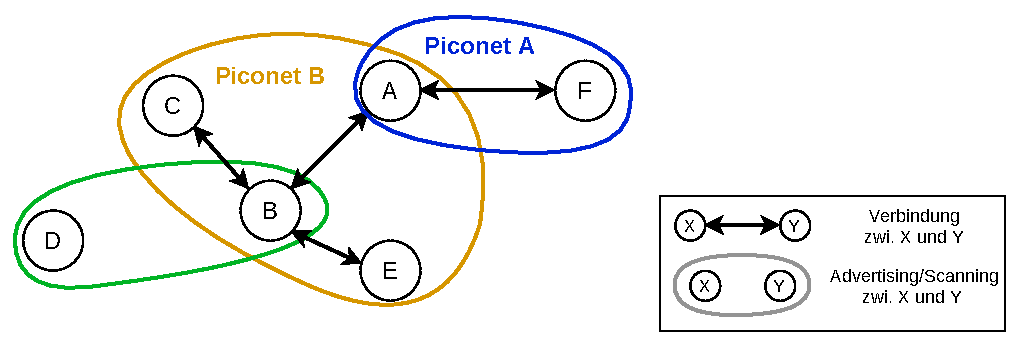
\includegraphics[width=0.6\textwidth]{graphics/le_topologie.pdf}
    \caption[Topologie in Low Energy]{Topologie in Low Energy}
    \label{fig: le topologie}
\end{figure}